%!TEX root = ../../thesis.tex
%*******************************************************************************
%****************************** Design Chapter *********************************
%*******************************************************************************

\chapter{Design}

\ifpdf
    \graphicspath{{Chapters/Design/Figs/}{Chapters/Design/Figs/}{Chapters/Design/Figs/}}
\else
    \graphicspath{{Chapters/Design/Figs/}{Chapters/Design/Figs/}}
\fi
The design of software systems is a critical aspect of \ac{se}, as it determines how the system will function and how well it will meet the needs of its users.
This chapter will discuss the Solution design explaining the Design Requirements of the solution (see section \ref{design:section:designReqs}), then concretize and codify them to establish some Design Principles (see section \ref{design:section:designprinciple}).
Then, in the next section, we design our tool using the LEAN development cycle phases containing Build (see section \ref{design:section:build}), Measure (see section \ref{design:section:measure}), and Learn (see section \ref{design:section:learn}).  
%********************************** % Solution Design **************************************
\section{Solution Design}
\label{design:section:soldesign}
To ensure that our study results can be applied to other contexts, we have created abstract design knowledge based on the \ac{dr}, codify our knowledge into \ac{dp} and the overall solution design.
%********************************** % Design Requirements **************************************
\subsection{Design Requirements}
\label{design:section:designReqs}
To derive a solution, we define some \ac{dr}s with the help of the literature review, state-of-the-art research, and comparing some tools.
In this context, each \ac{dr} refers to a generalized requirement that can be standardized and applied to future software applications. 
These requirements are abstract and cover a wide range of software needs.
We covered a wide range of topics including \textit{\ac{ui} Prototyping}, \textit{Low-Code/No-Code development}, \textit{Model-Based Software Engineering}, \textit{Continuous Experimentation}, \textit{Task-Based Usability Testing}, and the \textit{LEAN development process}.
The following section presents ten \ac{dr}s and their corresponding references in literature and tools. 
Moreover, most of the images used for the \ac{dr}s are taken from a website \textit{Webuild\footnote{Webuild: \url{https://webuild.io/why-use-figma-for-digital-product-design}}}.
% \paragraph*{Systematic literature reviews:} 
% Systematic literature reviews establish a solid basis for knowledge creation. 
% They help create theories and identify areas that require more research.
% By identifying existing literature and highlighting areas to explore, they also assist in the understanding of the problem space in DSR.
% Therefore, a comprehensive DSR project must include systematic literature reviews \cite{misc:dsr:webster}.
% \paragraph*{Interviews:}
% Interviews are regarded as empirical research to obtain primarily qualitative insights from individuals, such as specialists in a particular subject. 
% Suppose the interviewers are a part of the problem's stakeholder group.
% In that case, they may be utilized to establish requirements (or meta requirements) for the solution space that have a solid foundation for the problem space.
% For example, artifacts can be designed based on design principles (DPs) generated from interviews.
% Furthermore, the interviews can also be used to improve and evaluate the designed artifacts \cite{misc:dsr:mayring}. 
% \paragraph*{Other Methods:}
% Design requirements can also be generated using other methods or combinations of methods.
% Other methods include simulations, experiments, case studies, ethnography, and the grounded theory approach \cite{misc:dsr:nickerson, misc:dsr:varshney}. \\\\

\begin{figure}[htbp!]
  \centering    
  
\includegraphics[width=0.15\textwidth]{DR1.png}
  \caption[Heterogeneous Users]{\textbf{\ac{dr}1:} Heterogeneous Users}
  \label{fig:design:dr1}
\end{figure}
\textbf{\ac{dr}1: Involve Heterogeneous Users} states that \textit{The prototypes should support diverse users with different needs, goals, and capabilities and integrate internal and external users (see figure \ref{fig:design:dr1}).} 
In literature, this is reasoned by the fact that different users may have different needs, preferences, and levels of technical expertise \cite{misc:lean:steve}.
By including a diverse group of users, you can get a broader range of feedback and insights into how the software performs for different users \cite{article:prototyping:weichbroth}, simultaneously reducing the biases among developers \cite{misc:lean:burmeister}.
In this context, the users can be sourced from internal sources, such as employees, or external sources, like Amazon Mechanical Turk\footnote{Amazon Mechanical Turk: \url{https://www.mturk.com/}}.

\begin{figure}[htbp!]
  \centering    
  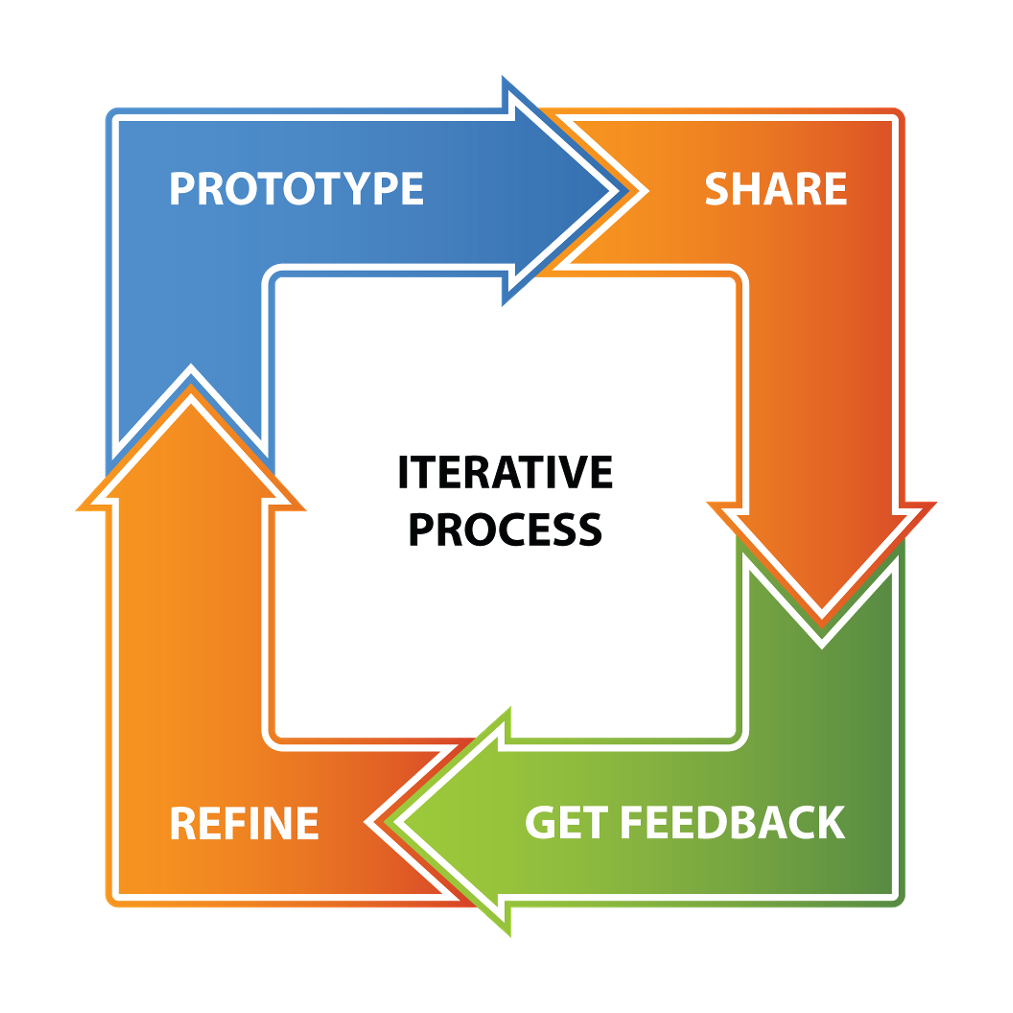
\includegraphics[width=0.15\textwidth]{DR2.png}
  \caption[Iterative approach development]{\textbf{\ac{dr}:} Iterative approach development}
  \label{fig:design:dr2}
\end{figure}
\textbf{\ac{dr}2: Iterative development approach} states that \textit{The prototypes should be developed in an iterative, incremental approach with some feedback mechanism in the end (see figure \ref{fig:design:dr2}).} 
In literature, this is reasoned by the fact that the iterative approach involves the idea of breaking down development into small, incremental cycles of work rather than trying to deliver a complete product all at once \cite{misc:lean:tutorial}.
The key benefit of an iterative approach is that it allows the development team to get feedback from users and stakeholders early in the development process and to make adjustments \cite{article:experiments:lindgren} to the product as needed.

\begin{figure}[htbp!]
  \centering    
  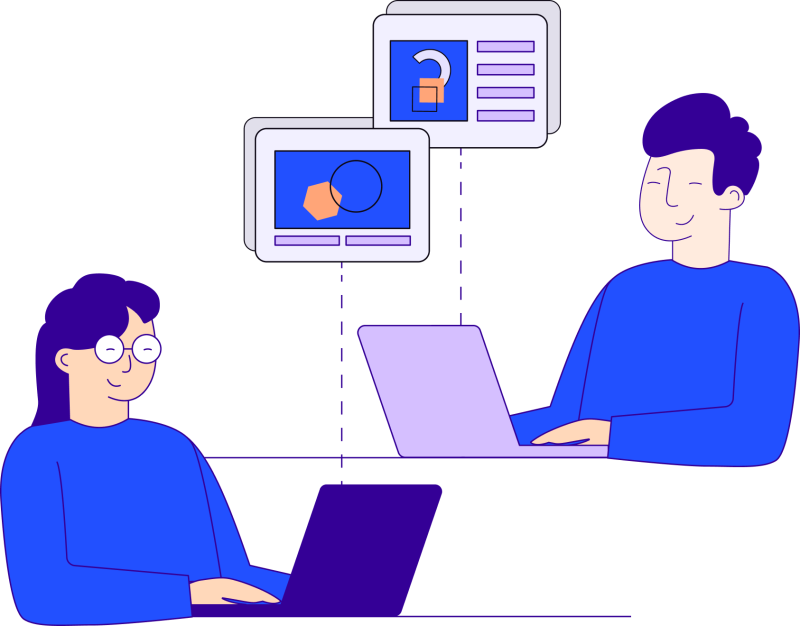
\includegraphics[width=0.15\textwidth]{DR3.png}
  \caption[Ease of use and intuitive]{\textbf{\ac{dr}3:} Ease of use and intuitive}
  \label{fig:design:dr3}
\end{figure}
\textbf{\ac{dr}3: Ease of use and intuitive} states that \textit{User-friendly, frictionless, fast and intuitive interfaces are essential for the prototypes helping the users improve the User Experience (\ac{ux}) of the prototype (see figure \ref{fig:design:dr3}).} 
In literature, this is reasoned by the fact that a tool should have easy navigation \cite{article:prototyping:hoffnagle}, clear and concise labels, icons, easy-to-use drag-and-drop functionality, collaboration capabilities (e.g., Figma\footnote{Figma Prototyping tool: \url{https://www.figma.com/}} has a feature where more than one person can access the prototype), and easily deployable \cite{article:prototyping:lowcode} features.
Various live examples like Figma, Invision\footnote{Invision: \url{https://www.invisionapp.com/}}, Axure\footnote{Axure Rapid Prototyping: \url{https://www.axure.com/}} have shown how user friendly and intuitive tools can have an impact on the users.

\begin{figure}[htbp!]
  \centering    
  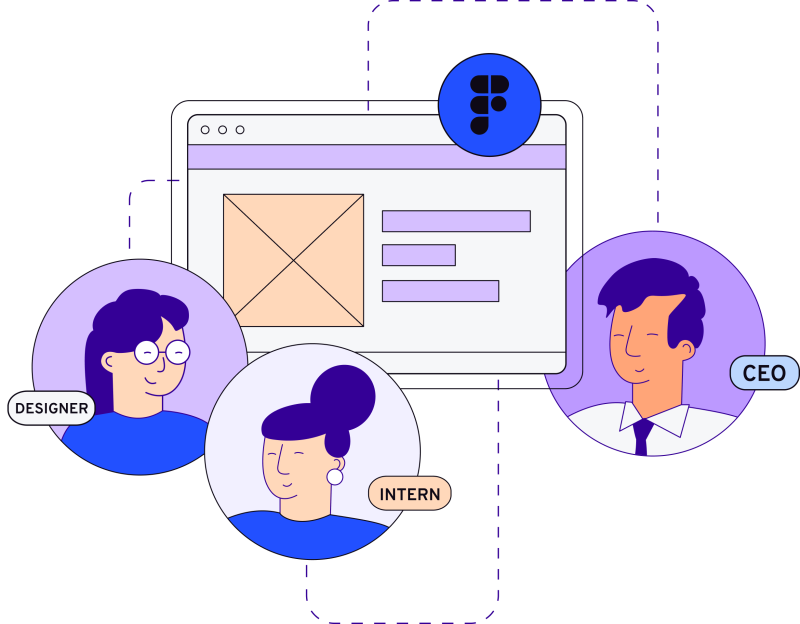
\includegraphics[width=0.15\textwidth]{DR4.png}
  \caption[Involve different stakeholders]{\textbf{\ac{dr}4:} Involve different stakeholders}
  \label{fig:design:dr4}
\end{figure}
\textbf{\ac{dr}4: Involve different stakeholders} states that \textit{Different stakeholders (e.g., designers, product managers, developers, etc.) should easily build the prototype, as each contribution is essential (see figure \ref{fig:design:dr4}).}
In literature, this is reasoned by the fact that involving different project stakeholders and providing them with the necessary communication tools helps exchange and codify knowledge \cite{article:prototyping:weichbroth}. 
This makes sure that the stakeholders' perspectives, requirements \cite{misc:prorotypes:lauff}, and their input helps shape the product's design.

\begin{figure}[htbp!]
  \centering    
  
\includegraphics[width=0.25\textwidth]{DR5.png}
  \caption[Design System]{\textbf{\ac{dr}5:} Atlassian example of a design system}
  \label{fig:design:dr5}
\end{figure}
\textbf{\ac{dr}5: Enhance design teamwork} states that \textit{There should be a live collaboration between the team members, and a full disclosure of the \ac{desy} of various disciplines making the tool easy for anyone to use on any platform and share their work quickly (see figure \ref{fig:design:dr5}).} 
A \texttt{\ac{desy}}\footnote{Design systems: \url{https://www.invisionapp.com/inside-design/guide-to-design-systems/}} is a collection of reusable components governed by some standards that can be assembled in many ways to make different applications.
In literature, this is reasoned by developers' ability to create more consistent, user-friendly prototypes that adhere to the design system's established style and principles \cite{paper:prototyping:luqi} and help improve the overall design process and product development \cite{article:prototyping:hoffnagle}.
In many tools, we saw the use of many design systems like \texttt{Design System Components} (e.g., buttons, forms, and icons, etc.), \texttt{Design System Patterns} (e.g., patterns for communication and data transfer between components, etc.), \texttt{Accessibility standards} (e.g., including some guidelines to promote accessibility and usability).

\begin{figure}[htbp!]
  \centering    
  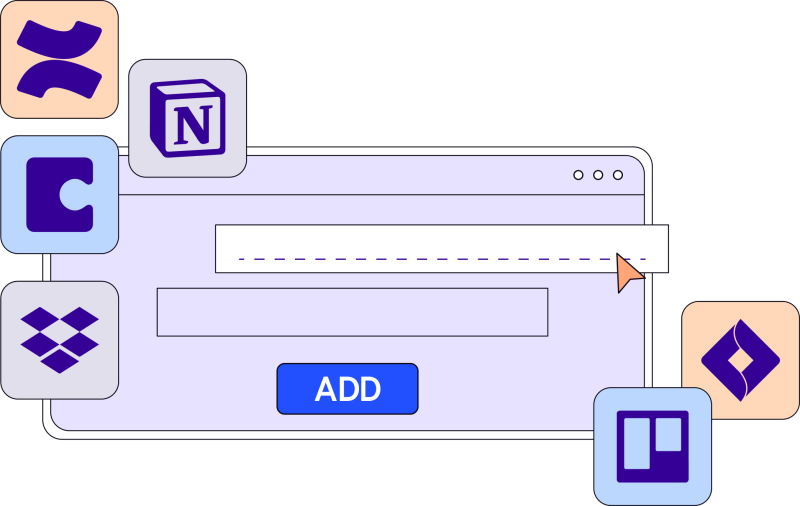
\includegraphics[width=0.2\textwidth]{DR6.png}
  \caption[Testing the prototype]{\textbf{\ac{dr}6:} Various methods to test the prototype}
  \label{fig:design:dr6}
\end{figure}
\textbf{\ac{dr}6: Diversity in testing} states that \textit{The prototype should be tested using various means by having users perform specific tasks and collect feedback called Task-based Usability tests (see figure \ref{fig:design:dr6}).} 
Testing of the \ac{gui} must be automated, and use functional and usability tests. 
Functional testing helps ensure the \ac{gui} works according to specification and usability testing helps ensure users can use the \ac{gui} effectively. 
And this helps in the identification and preliminary validation of user requirements in the early stages of development \cite{article:prototyping:weichbroth}.

\begin{figure}[htbp!]
  \centering    
  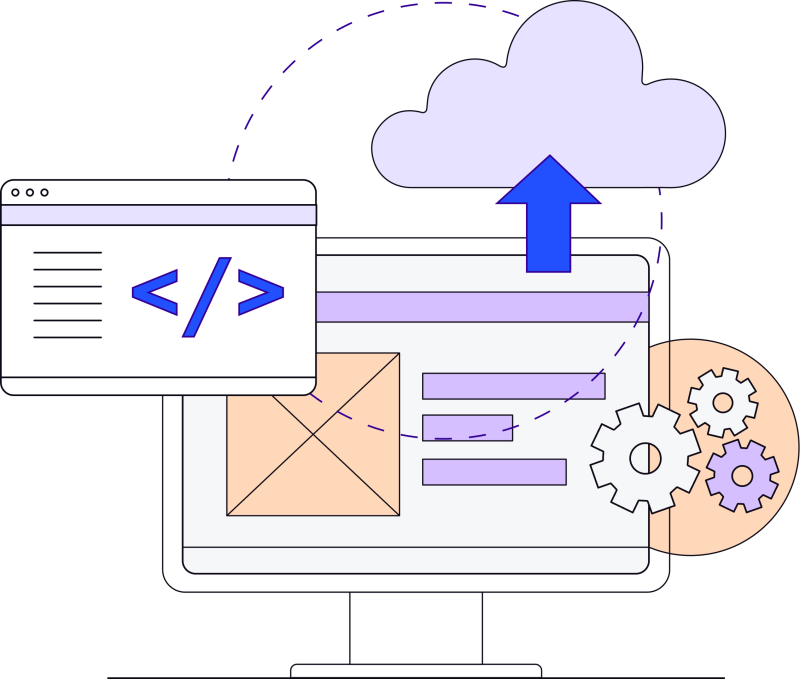
\includegraphics[width=0.15\textwidth]{DR7.png}
  \caption[Web-based tool]{\textbf{\ac{dr}7:} An auto-save web-based prototyping tool}
  \label{fig:design:dr7}
\end{figure}
\textbf{\ac{dr}7: An Auto-save Web-based prototyping tool} states that \textit{The tool should be a web-based application making it independent of any software, platforms (e.g., Macbooks, Windows \ac{pc}s, Linux machines, Chromebooks) and have an auto-save feature to store the work on Cloud (see figure \ref{fig:design:dr7}).}
In literature, this is reasoned by the fact that Web-based prototyping tools have several advantages \cite{misc:cloud} over traditional application-based tools.
In many tools like \texttt{Figma}, \texttt{Invision}, and \texttt{Axure}, we saw features\footnote{Some more features: \url{https://redrocksoftware.com.au/10-benefits-of-web-based-applications-systems/}} like \texttt{Accessibility} i.e., can be accessed from any device with an internet connection, \texttt{Collaboration} i.e., have built-in collaboration features, making it easy for team members to work on the same prototype simultaneously, \texttt{Updates} i.e., automatically updated.

% \textbf{DR9: Get user feedback} \textit{} Having users perform specific tasks and observe how they interact with the application helps improve the usability of the software applications. So, we can use task-based usability testing for achieving this. 
\begin{figure}[htbp!]
  \centering    
  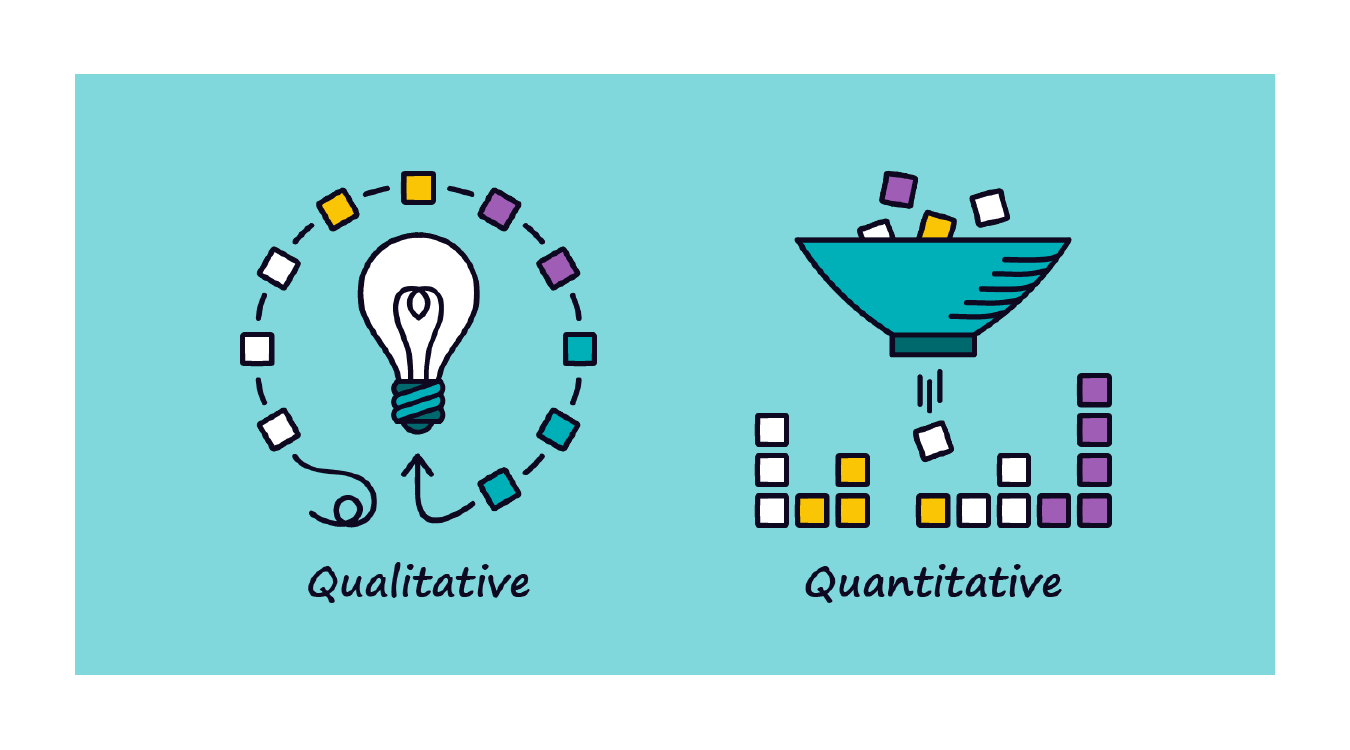
\includegraphics[width=0.2\textwidth]{DR8.png}
  \caption[Combine user feedbacks]{\textbf{\ac{dr}8:} A collaboration of qualitative and quantitative analysis}
  \label{fig:design:dr8}
\end{figure}
\textbf{\ac{dr}8: Combine user feedbacks} \textit{The prototype should gather user feedback and combine them to make improvements to the application.} 
In literature, this is reasoned by the fact that \texttt{Qualitative analysis} gathers an in-depth understanding of underlying reasons, opinions, and motivations \cite{misc:dsr:mayring}.
Whereas \texttt{Quantitative analysis} measures and understands numerical data and helps identify patterns and trends \cite{article:qqa:young}.
And together, qualitative and quantitative analysis can provide a more complete picture of a situation and can be used to validate or disprove findings from one type of analysis \cite{article:qq:helena}.

\begin{figure}[htbp!]
  \centering    
  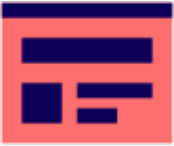
\includegraphics[width=0.1\textwidth]{DR9.png}
  \caption[Visualiza the Prototype]{\textbf{\ac{dr}9:} Visualiza the Prototype}
  \label{fig:design:dr9}
\end{figure}
\textbf{\ac{dr}9: Visualize the prototype} \textit{There should be a visualization tool for prototyping to help different stakeholders see and interact with the design and gather feedback.} 
In literature, this is reasoned by the fact that visualization helps in prototyping by allowing designers and stakeholders to see and understand the design in a way that is easy to understand \cite{article:comparative:prototypes}.
It also allows designers to identify usability issues \cite{article:prototyping:gould} early in the design process to make the end product user-friendly and easy to use.
In tools, various methods, like creating \texttt{Wireframes}\footnote{\textbf{Wireframe:} A wireframe is an essential visual representation of the layout and structure of a product, showing the placement of text, images, and buttons.}, \texttt{Mockups}\footnote{\textbf{Mockup:} A mockup is a more detailed version of a wireframe, typically created in color and with more realistic graphics and images.}, and \texttt{Interactive prototypes}\footnote{\textbf{Interactive Prototype:} An interactive prototype is a fully functional representation of a product, design, or feature.}, are used for visualization.

\begin{figure}[htbp!]
  \centering    
  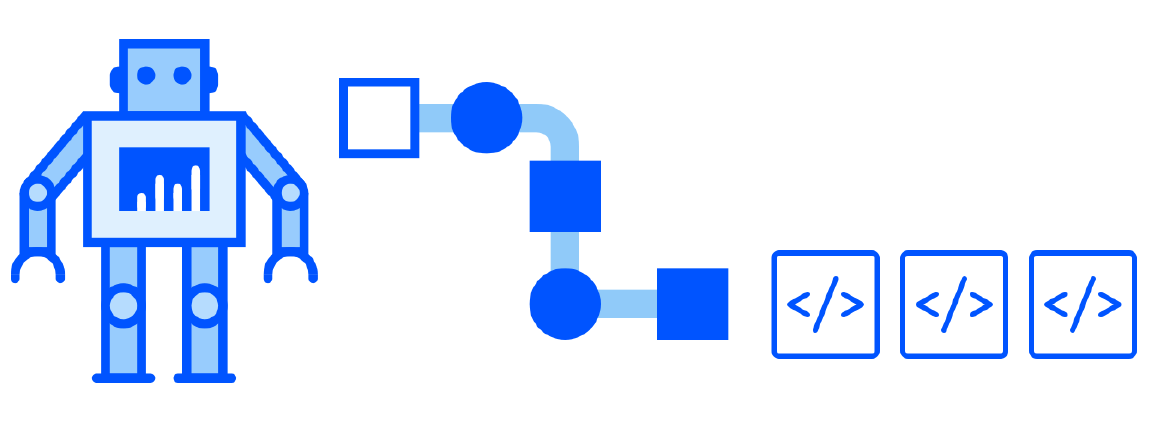
\includegraphics[width=0.2\textwidth]{DR10.png}
  \caption[Easy development]{\textbf{\ac{dr}9:} Development of any application should be easy}
  \label{fig:design:d10}
\end{figure}
\textbf{\ac{dr}10 Easy development:} \textit{A prototyping tool should be easily built and reduce the complexity.} 
In literature, this is reasoned by the fact that when software is easy to build, development teams can be more productive and efficient, leading to lower development costs \cite{misc:lowcode:platforms}. 
It's also easy for different development team members to understand and work on the code, thereby improving collaboration \cite{misc:prorotypes:lauff} and generating high-quality code.
Adding new features, scaling up, and making changes, as needed, make the tool more accessible and helpful \cite{article:prototyping:lowcode} to ensure that the tool remains relevant and valuable over time.


%********************************** % Design Principles **************************************
\subsection{Design Principles}
\label{design:section:designprinciple}
Design principles are guidelines or rules used to guide the design process in \ac{dsr} \cite{misc:dsr:henver}. 
They provide a framework for making design decisions \cite{paper:designprinciple:gregor} and help to ensure that the final solution meets the goals and objectives of the research. 
This section codifies our knowledge during the design study and derives \ac{dp}s from abstract \ac{dr}s from the iteration cycle of the \ac{dsr}.
The following shows the \textit{Eight \ac{dp}s} and references to literature and tools that build the foundation for the mapped \ac{dr}s (see figure \ref{fig:design:table-drs-dps}). 
\begin{figure}[htbp!]
  \centering    
  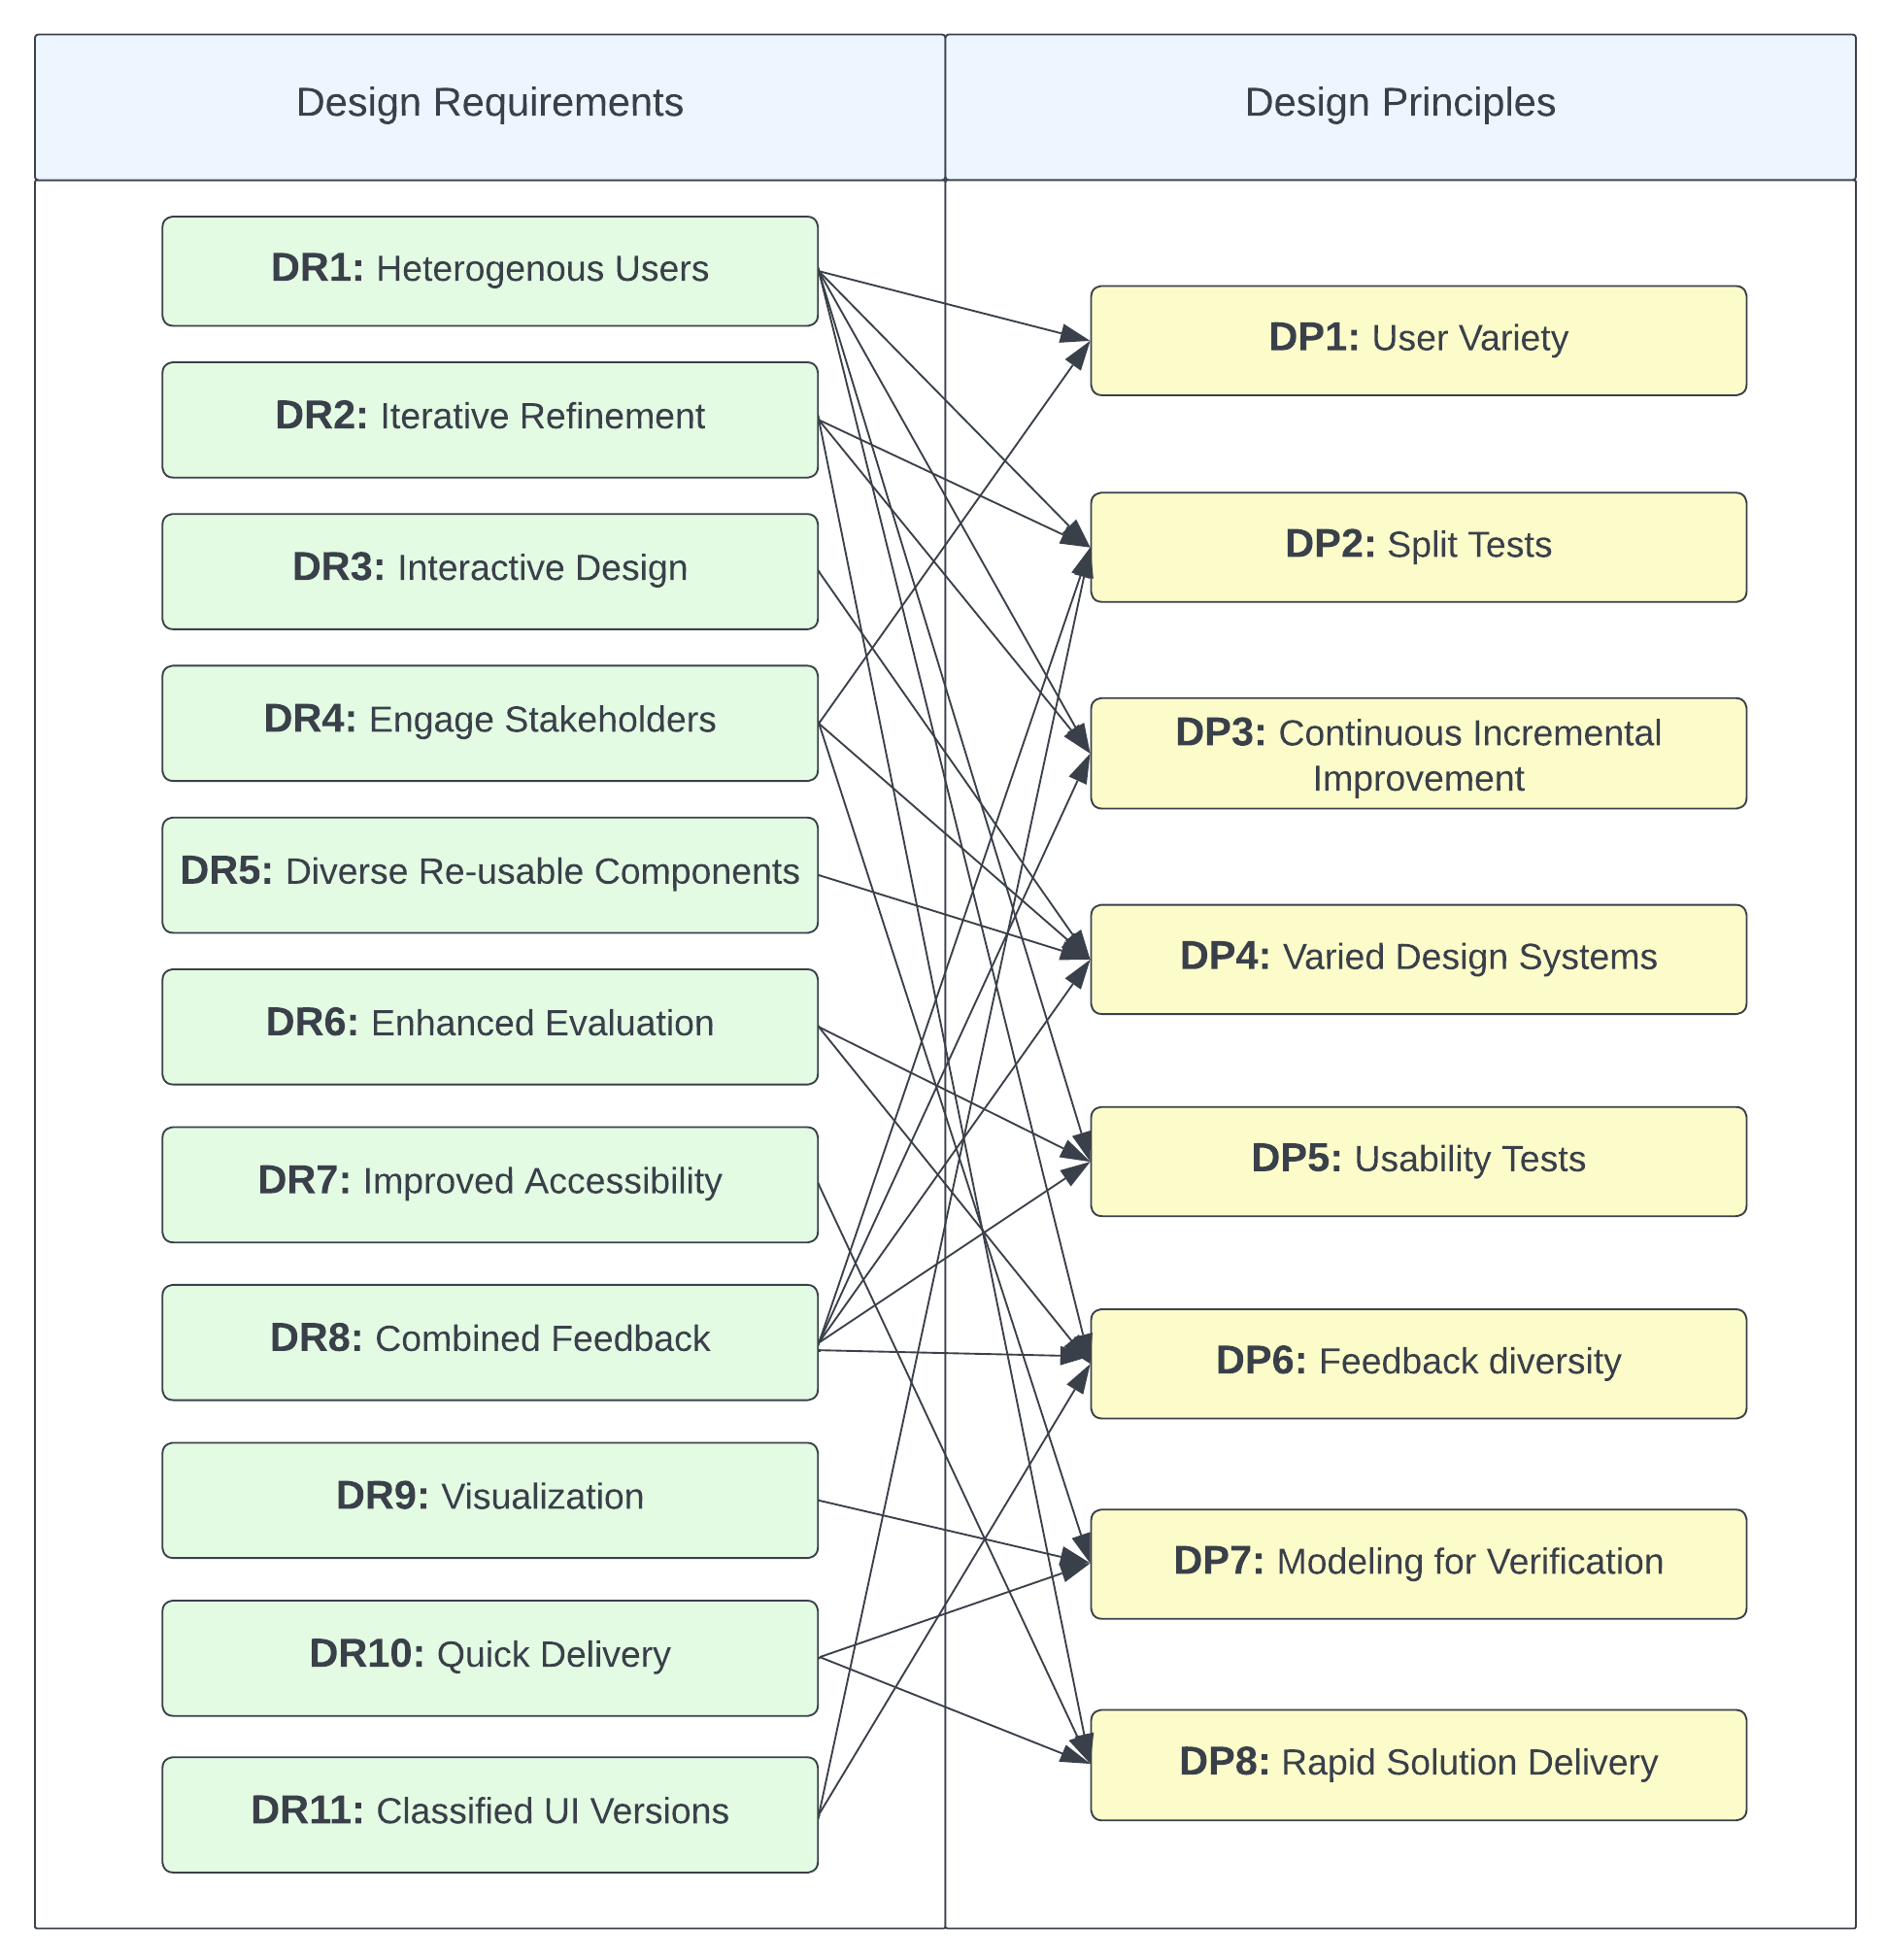
\includegraphics[width=0.9\textwidth]{Table-drs-dps.png}
  \caption[A map between \ac{dr}s and \ac{dp}s]{A map between Design Requirements and Design Principles}
  \label{fig:design:table-drs-dps}
\end{figure}

\paragraph{DP1: User Variety} \textit{}
\paragraph{DP2: Use Split Tests}
\paragraph{DP3: Continuous Improvement}
\paragraph{DP4: Involve different design systems}
\paragraph{DP5: Task-based tests}
\paragraph{DP6: Feedback diversity}
\paragraph{DP7: Modeling for verification}
\paragraph{DP8: Involve rapid development and platform independence}

\clearpage
%********************************** % Solution Concept **************************************
\section{Solution Concept}
\label{design:section:solutionconcept}

%********************************** % Build **************************************
\subsection{Build}
\label{design:section:build}

%********************************** % Measure **************************************
\subsection{Measure}
\label{design:section:measure}
%********************************** % Learn **************************************
\subsection{Learn}
\label{design:section:learn}